\documentclass[11pt, english, fleqn, DIV=15, headinclude, BCOR=1cm]{scrartcl}

\usepackage[bibatend]{../header}

\usepackage{lastpage}
\usepackage{multicol}
\usepackage{simplewick}
\usepackage{slashed}
\usepackage{subcaption}
\usepackage{minted}

\newcommand\timeorder{\mathscr T}
\newcommand\normorder{\mathscr N}
\newcommand\eye{\mat 1_4}
\newcommand\myslash[1]{\underline{\slashed{\vec{#1}}}}

\hypersetup{
    pdftitle=
}

\graphicspath{{build/}}

\newcounter{totalpoints}
\newcommand\punkte[1]{#1\addtocounter{totalpoints}{#1}}

\newcounter{problemset}
\setcounter{problemset}{4}

\subject{physics617 -- Theoretical Condensed Matter Physics}
\ihead{physics617 -- Problem Set \arabic{problemset}}

\title{Problem Set \arabic{problemset}}

\newcommand\thegroup{Tutor: Ramsés Sánchez}

\publishers{\thegroup}
\ofoot{\thegroup}

\author{
    Martin Ueding \\ \small{\href{mailto:mu@martin-ueding.de}{mu@martin-ueding.de}}
}
\ifoot{Martin Ueding}

\ohead{\rightmark}

\begin{document}

\maketitle

\vspace{3ex}

\begin{center}
    \begin{tabular}{rrr}
        \toprule
        Problem & Achieved points & Possible points \\
        \midrule
        \nameref{homework:1} & & \punkte{15} \\
        \nameref{homework:2} & & \punkte{5} \\
        \nameref{homework:3} & & \punkte{10} \\
        \midrule
        Total & & \arabic{totalpoints} \\
        \bottomrule
    \end{tabular}
\end{center}

\vspace{3ex}

\begin{center}
    \begin{small}
        This document consists of \pageref{LastPage} pages.
    \end{small}
\end{center}

\section{The $\mathrm{CuO_2}$ lattice}
\label{homework:1}

There must be one oxygen atom missing in Figure~1 on the problem set. Otherwise
the unit cell would be more complex and would contain more than three atoms.
The wording with the lattice spacing is not completely clear to me. I will now
assume that the distance between neighboring O and Cu atoms is $a$ as shown in
Figure~\ref{fig:cuo-unit-cell}.

\begin{figure}
    \centering
    \includegraphics{cuo-unit-cell}
    \caption{%
        Unit cell of $\mathrm{CuO_2}$.
    }
    \label{fig:cuo-unit-cell}
\end{figure}

\newcommand\ed{\epsilon_\mathrm d}
\newcommand\ep{\epsilon_\mathrm p}

We are given the tight-binding Hamiltonian
\begin{align*}
    H
    &= \sum_{\vec j, \sigma} \left[
        \ed d_{\vec j, \sigma}^\dagger d_{\vec j, \sigma}
        + \ep \sbr {
            p_{1 \, \vec j, \sigma}^\dagger p_{1 \, \vec j, \sigma}
            p_{2 \, \vec j, \sigma}^\dagger p_{2 \, \vec j, \sigma}
        }
        \right.
        \\&\quad
        \left.
        - t \sbr{
            d_{\vec j, \sigma}^\dagger p_{1 \, \vec j, \sigma}
            + d_{\vec j, \sigma}^\dagger p_{2 \, \vec j, \sigma}
            + d_{\vec j + \vec y, \sigma}^\dagger p_{1 \, \vec j, \sigma}
            + d_{\vec j + \vec x, \sigma}^\dagger p_{2 \, \vec j, \sigma}
        }
    \right] + \hc \,.
    \intertext{%
        In order to say anything about the band structure, we need to represent
        this in some momentum basis. We do this again by a simple Fourier
        transform with
        \[
            c_{\vec x, l} = \frac{1}{\sqrt{N_\mathrm c}} \sum_{\vec k} c_{\vec
            k, l} \exp(\iup \vec k \cdot [\vec x + \vec r_l])
        \]
        for the position space ladder operators. We call the copper lattice
        site “0”, the first p-orbital “1” and the second p-orbital “2” within
        the unit cell. Inserting all this will give us a very long Hamiltonian.
    }
    H &= \frac1{N_\mathrm c} \sum_{\vec j, \sigma} \sum_{\vec k, \vec k'} \left[
    \ed c_{\vec k' 0}^\dagger c_{\vec k 0}
    \exp(-\iup \vec k' \cdot [\vec j + \vec 0])
    \exp(\iup \vec k \cdot [\vec j + \vec 0])
    \right.
    \\&\quad
    +
    \ep c_{\vec k' 1}^\dagger c_{\vec k 1}
    \exp(-\iup \vec k' \cdot [\vec j + \vec y/2])
    \exp(\iup \vec k \cdot [\vec j + \vec y/2])
    \\&\quad
    +
    \ep c_{\vec k' 2}^\dagger c_{\vec k 2}
    \exp(-\iup \vec k' \cdot [\vec j + \vec x/2])
    \exp(\iup \vec k \cdot [\vec j + \vec x/2])
    \\&\quad
    -
    t c_{\vec k' 0}^\dagger c_{\vec k 1}
    \exp(-\iup \vec k' \cdot [\vec j + \vec 0])
    \exp(\iup \vec k \cdot [\vec j + \vec y/2])
    \\&\quad
    -
    t c_{\vec k' 0}^\dagger c_{\vec k 2}
    \exp(-\iup \vec k' \cdot [\vec j + \vec 0])
    \exp(\iup \vec k \cdot [\vec j + \vec x/2])
    \\&\quad
    -
    t c_{\vec k' 0}^\dagger c_{\vec k 1}
    \exp(-\iup \vec k' \cdot [\vec j + \vec 0])
    \exp(\iup \vec k \cdot [\vec j + \vec y/2])
    \\&\quad
    \left.
    -
    t c_{\vec k' 0}^\dagger c_{\vec k 2}
    \exp(-\iup \vec k' \cdot [\vec j + \vec y + \vec 0])
    \exp(\iup \vec k \cdot [\vec j + \vec x + \vec x/2])
    \right] + \hc
    \intertext{%
        The two exponentials each can be joined. The terms with $\vec j$ in
        both exponentials will, together with $\sum_{\vec j}$ and the
        $1/N_\mathrm c$, give a $\delta(\vec k - \vec k')$. We remove the
        $\sum_{\vec k'}$ using that $\delta$ right away. The remainder of the
        exponentials will stay there with $\vec k = \vec k'$. Then we end up
        with
    }
    H &= \sum_{\sigma} \sum_{\vec k}
    \left[
    \ed c_{\vec k 0}^\dagger c_{\vec k 0}
    + \ep \sbr{c_{\vec k 1}^\dagger c_{\vec k 1} + c_{\vec k 2}^\dagger c_{\vec k 2}}
    \right.
    - t c_{\vec k 0}^\dagger c_{\vec k 1}
    \exp(\iup \vec k \cdot \vec y/2)
    - t c_{\vec k 0}^\dagger c_{\vec k 2}
    \exp(\iup \vec k \cdot \vec x/2)
    \\&\quad
    \left.
    - t c_{\vec k 0}^\dagger c_{\vec k 1}
    \exp(- \iup \vec k \cdot \vec y/2)
    - t c_{\vec k 0}^\dagger c_{\vec k 2}
    \exp(- \iup \vec k \cdot \vec x/2)
    \right] + \hc \,.
    \intertext{%
        The last four terms can be joined into two terms with a cosine
        contribution. Then our final form is
    }
    H &= \sum_{\sigma} \sum_{\vec k}
    \sbr{
        \ed c_{\vec k 0}^\dagger c_{\vec k 0}
        + \ep \sbr{c_{\vec k 1}^\dagger c_{\vec k 1} + c_{\vec k 2}^\dagger c_{\vec k 2}}
        - 2 t c_{\vec k 0}^\dagger c_{\vec k 1}
        \cos(\iup \vec k \cdot \vec y/2)
        - 2 t c_{\vec k 0}^\dagger c_{\vec k 2}
        \cos(\iup \vec k \cdot \vec x/2)
    } \\&\quad + \hc \,.
    \intertext{%
        To diagonalize the Hamiltonian it is convenient to write it in matrix
        form with the three ladder operators that we have.
    }
    H &= 2 \sum_{\sigma} \sum_{\vec k}
    \begin{pmatrix}
        c_{\vec k 0} \\ c_{\vec k 1} \\ c_{\vec k 2}
    \end{pmatrix}^\dagger
    \begin{pmatrix}
        \ed & -t \cos(\vec k \cdot \vec y/2) & -t \cos(\vec k \cdot \vec x/2) \\
        -t \cos(\vec k \cdot \vec y/2) & \ep & 0 \\
        -t \cos(\vec k \cdot \vec x/2) & 0 & \ep
    \end{pmatrix}
    \begin{pmatrix}
        c_{\vec k 0} \\ c_{\vec k 1} \\ c_{\vec k 2}
    \end{pmatrix}
    \intertext{%
        The vectors $\vec x$ and $\vec y$ are of length $a$ and in the $x$ and
        $y$ direction. Therefore the scalar products simplify to the components
        of $\vec k$.
    }
    H &= 2 \sum_{\sigma} \sum_{\vec k}
    \begin{pmatrix}
        c_{\vec k 0} \\ c_{\vec k 1} \\ c_{\vec k 2}
    \end{pmatrix}^\dagger
    \begin{pmatrix}
        \ed & -t \cos(k_y) & -t \cos(k_x) \\
        -t \cos(k_y) & \ep & 0 \\
        -t \cos(k_x) & 0 & \ep
    \end{pmatrix}
    \begin{pmatrix}
        c_{\vec k 0} \\ c_{\vec k 1} \\ c_{\vec k 2}
    \end{pmatrix}
\end{align*}

Then again we diagonalize this matrix using \emph{Mathematica} and retrieve the
eigenvalues
\[
    \lambda_1 = \ep
    \eqnsep
    \lambda_\pm
    = \frac{\ep + \ed}{2} \pm \sqrt{
        \sbr{\frac{\ed - \ep}{2}}^2
        + t^2 + \frac{t^2}{2} \sbr{\cos(2 k_x) + \cos(2 k_y)}
    } \,.
\]

Those eigenvalues are visualized in Figure~\ref{fig:eigenvalues}.

\begin{figure}
    \centering
    \begin{subfigure}[t]{0.48\linewidth}
        \centering
        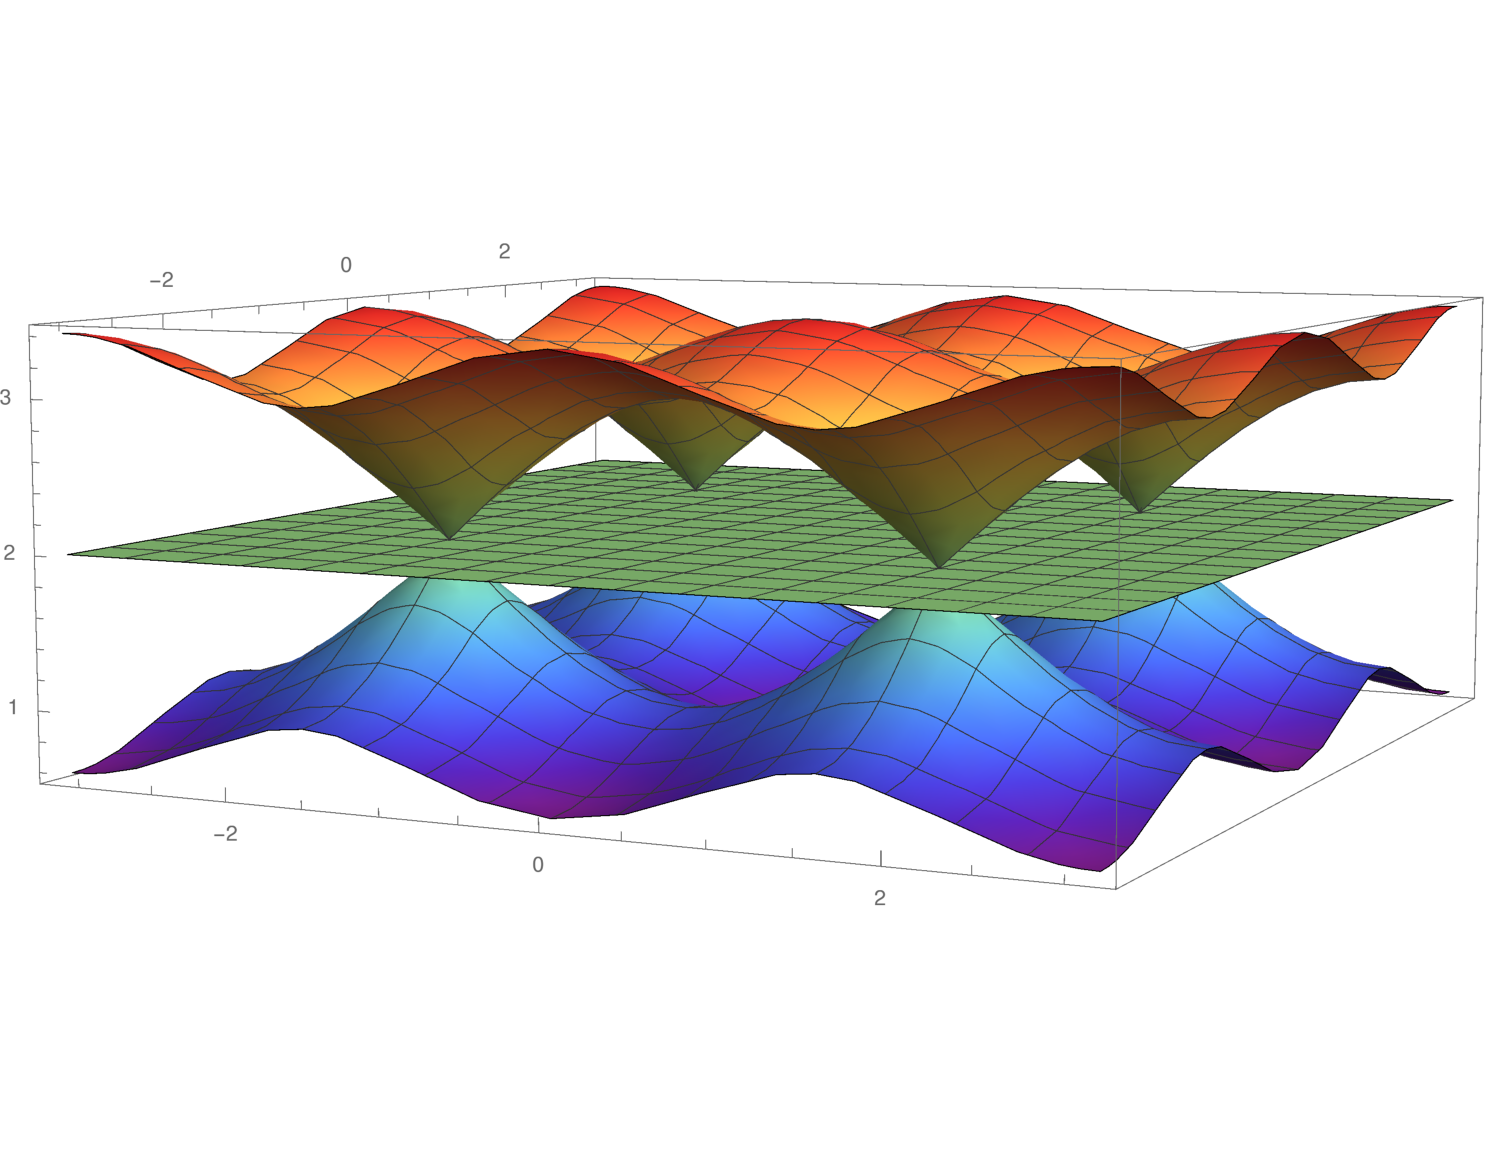
\includegraphics[width=\linewidth]{1_1_1.pdf}
        \caption{%
            $\ed = \num{1}$,
            $\ep = \num{1}$,
            $t = \num{1}$. There is no gap between the three bands.
        }
        \label{fig:eigenvalues/1}
    \end{subfigure}
    \hfill
    \begin{subfigure}[t]{0.48\linewidth}
        \centering
        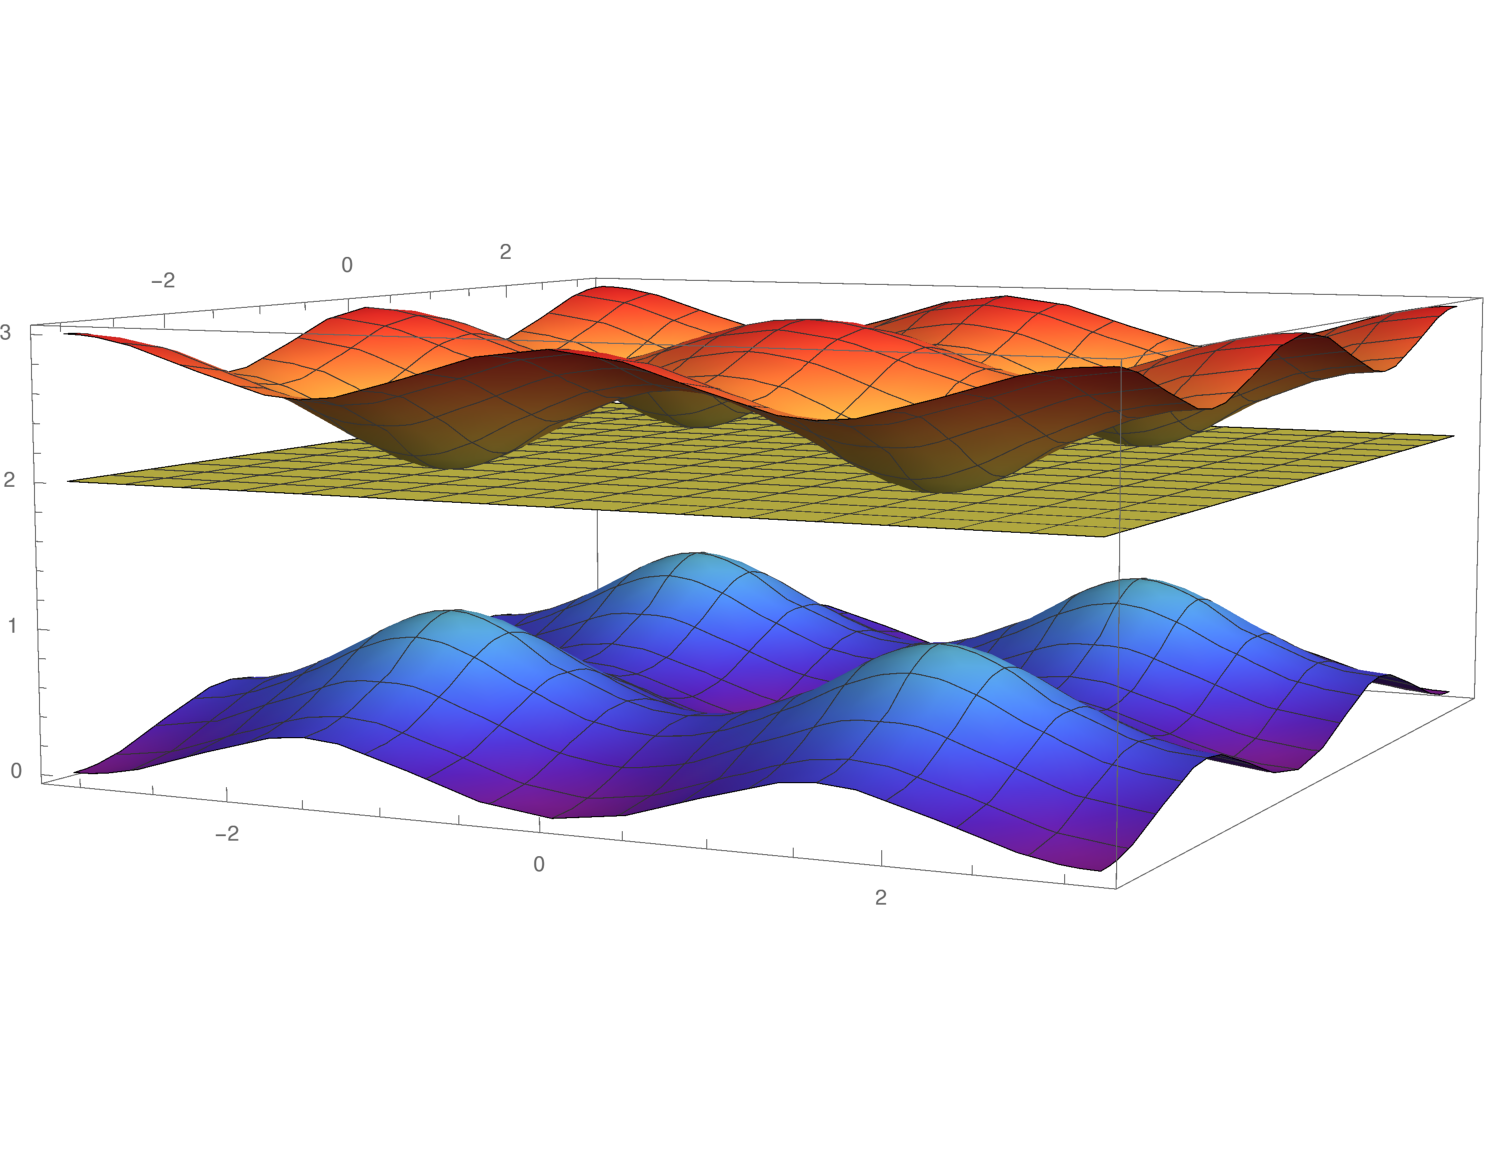
\includegraphics[width=\linewidth]{05_1_1.pdf}
        \caption{%
            $\ed = \num{1}$,
            $\ep = \num{0.5}$,
            $t = \num{1}$. One can see how a band gap between the two
            interesting bands occurs.
        }
        \label{fig:eigenvalues/2}
    \end{subfigure}
    \caption{%
        Band structure of the $\mathrm{CuO_2}$ lattice plotted against $a k_x$
        and $a k_y$ in the Brillouin zone. Shown are all three bands with a
        rainbow color scheme for the energy.
    }
    \label{fig:eigenvalues}
\end{figure}

\section{Density of states for hybridized bands}
\label{homework:2}

\section{Density of states of a phonon mode of a 2D system}
\label{homework:3}

\subsection{Numerical computation}

A dispersion
\[
    E(\vec k) \propto \sqrt{2 - \cos(k_x) - \cos(k_y)}
\]
is given. The energy values lie in the interval $[0, 2]$. The wave vectors
$\vec k$ lie in the first Brillouin zone which is $(-\piup, \piup]^2$ here. Due
to the symmetry of the dispersion relation it suffices to iterate in the
interval $[0, \piup]^2$.

The dispersion relation is illustrated in Figure~\ref{fig:dispersion}. The
contour plot in Figure~\ref{fig:dispersion/2} makes it clear that there are
some straight contour lines. At those points the gradient vanishes in one
direction which will give rise to an peak in density of states.

\begin{figure}
    \centering
    \begin{subfigure}[c]{0.48\linewidth}
        \centering
        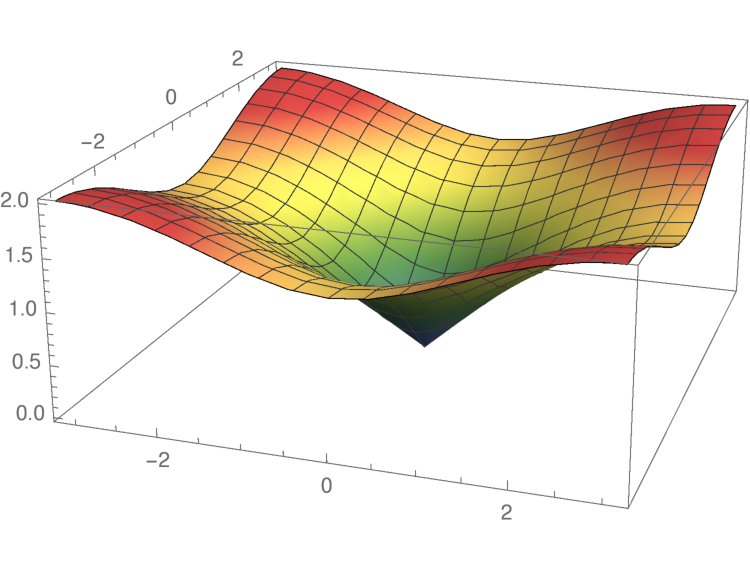
\includegraphics[width=\linewidth]{dispersion.pdf}
        \caption{%
            3D plot, energy versus wave vectors.
        }
        \label{fig:dispersion/1}
    \end{subfigure}
    \hfill
    \begin{subfigure}[c]{0.48\linewidth}
        \centering
        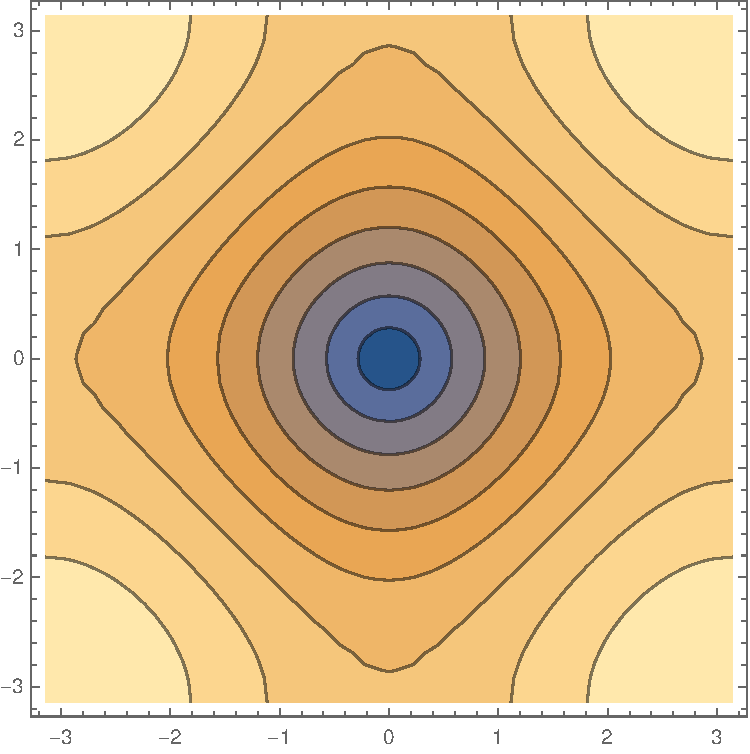
\includegraphics[width=\linewidth]{contour.pdf}
        \caption{%
            Contour plot, energy versus wave vectors.
        }
        \label{fig:dispersion/2}
    \end{subfigure}
    \caption{%
        Dispersion relation in two different plot variants. Both were made with
        \emph{Mathematica} as \emph{pgfplots} has a hard time with 3D plots.
    }
    \label{fig:dispersion}
\end{figure}

We haven chosen the approach to sample a grid in the interval $[0, \piup]^2$
and compute the energy for each of those wave vectors. Then we build up a
histogram with the energies. The resulting distribution is the density of
states with respect to the energy.

Listing~\ref{lst:cpp} shows the C++ version of it. Except for the use of the
brace initialization and \texttt{auto} this would compile with the C++03
standard. But why use that when one has two C++14 compliant compilers on the
system? It uses a simple histogram implementation which is enough for this
application. After the sampling of the grid it will scale the histogram counts
such that the end result is a proper density function with unit integral.
Listing~\ref{lst:cmake} shows the short CMake file to compile the program.

\begin{listing}[tb]
    \inputminted[linenos, fontsize=\footnotesize]{cpp}{dos.cpp}
    \caption{%
        C++ program for density of state computation.
    }
    \label{lst:cpp}
\end{listing}

\begin{listing}[tb]
    \inputminted[linenos, fontsize=\footnotesize]{cmake}{CMakeLists.txt}
    \caption{%
        CMake build file for C++ program.
    }
    \label{lst:cmake}
\end{listing}

We implemented the same algorithm again in Python with the NumPy and SciPy
libraries. This is shown in Listing~\ref{lst:python}. In order to benefit from
the native implementation of the NumPy routines we have chosen not to iterate
the grid with Python itself but using 2D arrays of the grid points. As a last
step we compute the integral of the density function to make sure that the
integral is approximately unity.

\begin{listing}[tb]
    \inputminted[linenos, fontsize=\footnotesize]{python}{dos.py}
    \caption{%
        Python program for density of state computation.
    }
    \label{lst:python}
\end{listing}

The results of both programs are shown in Figure~\ref{fig:dos-numerical}. The
C++ version was run with a lot more sampling points and more bins. Therefore it
is not surprising that the result looks better.

\begin{figure}
    \centering
    \includegraphics{dos-numerical}
    \caption{%
        Numerical density of states function with analytic approximation.
    }
    \label{fig:dos-numerical}
\end{figure}

The peak at around $\epsilon/\omega_0 = \num{1.4}$ arises from the parts of the
dispersion without curvature. The vanishing of curvature can be seen as
straight contour lines on Figure~\ref{fig:dispersion/2}.

\subsection{Analytical approximation}

Here we are supposed to use the approximation
\[
    \omega = \omega_0 \frac{|\vec k|}{\sqrt 2} \,.
\]
We can compute the density of states using the definition:
\begin{align*}
    \rho(\epsilon)
    &= \frac{2}{N} \sum_{\vec k} \delta(\epsilon - \epsilon(\vec k)) \,.
    \intertext{%
        We need to write this as an integral in two dimensional volume $V$.
    }
    &= \frac{V}{[2 \piup]^2} \int \dif^2 k \,
    \delta(\epsilon-\epsilon(\vec k))
    \intertext{%
        With the explicit approximation this integral becomes
    }
    &= \frac{V}{[2 \piup]^2} \int \dif^2 k \,
    \delta\del{\epsilon-\frac{\omega_0}{\sqrt{2}} \sqrt{k_1^2 + k_2^2}} \,.
    \intertext{%
        Now we change to polar coordinates to make this solvable. We directly
        perform the $\phi$ integral which gives us a factor of $2 \piup$.
    }
    &= \frac{V}{2 \piup} \int \dif k \, k
    \delta\del{\epsilon-\frac{\omega_0}{\sqrt{2}} k} \,.
    \intertext{%
        Another change of variables will move the factor out front.
    }
    &= \frac{V}{\omega_0 \piup} \int \dif \kappa \, \kappa
    \delta(\epsilon- \kappa)
    \intertext{%
        The result is easy, we just have
    }
    &= \frac{V}{\omega_0 \piup} \epsilon \,.
\end{align*}
In order to have a proper density function we need to normalize this to be
\[
    \rho(\epsilon) = \frac 12 \epsilon \,.
\]
We cannot compare this to the numerical result, though. Therefore we use the
same form with $V = 1$ and $\omega_0 = 1$ and have
\[
    \rho(\epsilon) = \frac 1\piup \epsilon.
\]
This is also shown in Figure~\ref{fig:dos-numerical}.


\end{document}

% vim: spell spelllang=en tw=79
